\documentclass{article}
\usepackage[T2A]{fontenc} 
\usepackage[utf8]{inputenc} 
\usepackage[english,russian]{babel}
\usepackage{graphicx} 
\usepackage{amsmath}
\usepackage{amsfonts} 
\usepackage{titlesec}
\usepackage{listings}
\usepackage{float}
\usepackage{longtable}
\usepackage{titling} 
\usepackage{geometry} 
\usepackage{pgfplots}
\pgfplotsset{compat=1.9}
\usepackage{xcolor}
\definecolor{darkgreen}{RGB}{0,100,0}

\lstset{
  language=Python,
  basicstyle=\ttfamily,
  keywordstyle=\color{darkgreen},
  stringstyle=\color{purple},
  commentstyle=\color{green},
  morecomment=[l][\color{magenta}]{\#},
  frame=single, 
  showspaces=false, 
  showstringspaces=false, 
  numbers=left, 
  numberstyle=\tiny,
}

\titleformat{\section}
  {\normalfont\Large\bfseries}{\thesection}{1em}{}
\titleformat{\subsection}
  {\normalfont\large\bfseries}{\thesubsection}{1em}{}

\setlength{\droptitle}{-6em} 
\title{Отчет по лабораторной работе № 3\\ Вариант № 3}
\author{Винницкая Дина Сергеевна}
\date{Группа: Б9122-02-03-01сцт}

\geometry{a4paper, margin=2cm}

\begin{document}

\maketitle
\section*{Цель работы}
\begin{enumerate}
    \item Реализовать формулу дифференцирования с учётом равномерной сетки для порядка первой производной;
    \item Получить значения $\min{R}$ и $\max{R}$ для остаточного члена R;
    \item Проверить выполнение неравентсва $\min{R} < R(x_m) < \max(R)$ где $x_m - $ заданный узел
    \item Сделать вывод по проделанной работе.
\end{enumerate}

\section*{Входные данные:}
\begin{enumerate}

    \item \textbf{Функция:} $y=x^2 + \ln(x) - 4$
    \item \textbf{Отрезок} $[1.5,2.0]$
    \item $n = 3; \quad k = 1; \quad m = 2;$
    
\end{enumerate}

\section*{Ход работы:}

\section{Вывод первой производной по методу Лагранжа}
Из указанной в методической книжке таблицы, необходимо вычислислить первую производную:
\[
L_n(x) = \sum \limits_{i = 0}^n f(x_i) \prod \limits_{j = 0;\ j \neq i}^n (x - x_j)
\]
\[
L'_n(x) = \sum \limits_{i = 0}^n f(x_i) \prod \limits_{j = 0;\ j \neq i}^n \dfrac 1 {x_i - x_j} \cdot \dfrac d {dx} \prod \limits_{j = 0;\ j \neq i}^n (x - x_j) = \sum \limits_{i = 0}^n f(x_i) \prod \limits_{j = 0;\ j \neq i}^n \dfrac 1 {x_i - x_j} \cdot \left(\sum \limits^n_{j = 0;\ j \neq i}\ \prod \limits_{
\begin{subarray}{l}
\mathsf{j_1 = 0}\\
\mathsf{j_1 \neq j \neq i}
\end{subarray}
}^n (x - x_{j_1})\right)
\]
\[
L'_n(x_m) = \sum \limits_{i = 0}^n \dfrac{f(x_i)}{h} \prod \limits^n_{
\begin{subarray}{l}
\mathsf{j = 0} \\
\mathsf{j \neq i}
\end{subarray}}
\dfrac 1 {i - j} \cdot \left(\sum \limits_{j = 0}^n \prod \limits_{
\begin{subarray}{l}
\mathsf{j1 = 0} \\
\mathsf{j1 \neq j \neq i}
\end{subarray}
}^n (m - j) \right)
\]

\section{Используемые библиотеки}
Для реализации необходимой программы используются следующие библиотеки языка Python:


\begin{itemize}
    \item \textbf{sympy} - библиотека $\textbf{sympy}$ представляет собой мощный символьный математический пакет для $\textbf{Python}$. Она способна обрабатывать символьные выражения, уравнения, и действия, что делает ее полезным инструментом в области научных вычислений, анализа данных и математического моделирования.
    \begin{itemize}
        \item \textbf{Функциональность:} библиотека $\textbf{sympy}$ позволяет выполнять различные операции с символами, такие как дифференцирование, интегрирование, решение уравнений и многое другое, что делает ее важным ресурсом для работы с математическими вычислениями в $\textbf{Python}$.
    \end{itemize}
\end{itemize}
\begin{itemize} \item \textbf{math} - библиотека 
math
 в Python предоставляет функции для выполнения математических операций над числами. Она включает в себя функции для работы с простыми и сложными математическими операциями, такими как тригонометрия, логарифмы, округления чисел и т.д. \begin{itemize} \item \textbf{Функциональность:} Библиотека 
math
 предоставляет широкий спектр математических функций, которые могут использоваться для решения различных задач, как в научных и инженерных вычислениях, так и в разработке программного обеспечения. 
 \end{itemize} 
 \end{itemize}

\begin{lstlisting}
import sympy as sp
import math
\end{lstlisting}


\section{Инициализация входных данных}
Начиная реализацию алгоритма известна непосредственная функция$y=x^2 + \ln(x) - 4$ и отрезок $[1.5,2.0]$ \

\begin{lstlisting}
    x = sp.symbols('x')
    n = 3
    k = 1
    m = 2
    a = 1.5
    b = 2.0
    step = (b - a) / 3
    points = values(a, b, step)
    L = lagrange_polynomial(points, x)
\end{lstlisting}

\begin{lstlisting}
def func(x):
    return x ** 2 + sp.log(x) - 4
\end{lstlisting}

\section{Реализация основного алгоритма}
\textbf{\large{Создание таблицы значений функции}}
\begin{lstlisting}
def values(a, b, step):
    table = []
    x = a
    
    while x <= b:
        table.append((x, func(x)))
        x += step
        
    return table
\end{lstlisting}
\begin{itemize}
\item Функция \textbf{ values(a, b, step)} создает таблицу значений функции на заданном интервале. Результатом является список кортежей, представляющих пары \textbf{ (x, f(x))}, где \textbf{x} - значения аргумента, а \textbf{f(x) }- соответствующие значения функции на этом аргументе.
\end{itemize}

\textbf{\large{Таблица значений функции}}

\begin{center}

\begin{tabular}{|c|c|} 
\hline
x & y(x) \\
\hline
1.5 & -1.34453489189184 \\
\hline
1.6666666666666667 & -0.711396598456231 \\
\hline
1.8333333333333335 & -0.0327530853185727 \\
\hline
2.0 & 0.693147180559945 \\
\hline
\end{tabular}
\end{center}


$\\ \\ \\ \\ \\ $

\textbf{\large{Вычисление многочлена Лагранжа}}
\begin{lstlisting}
def lagrange_polynomial(points, x):
    l = 0
    for i, (x_i, y_i) in enumerate(points):
        l_i = 1
        for j, (x_j, _) in enumerate(points):
            if i != j:
                l_i *= (x - x_j) / (x_i - x_j)
        l += y_i * l_i
    return l
\end{lstlisting}
\begin{itemize}
\item Функция $\textbf{lagrange\_polynomial(points, x)}$ вычисляет многочлен Лагранжа для заданных точек. Она принимает список точек $(x_i, y_i)$ и аргумент \textbf{x}, для которого необходимо вычислить значение многочлена. 
\end{itemize}
\textbf{\large{Вывод}} \\
$-1.34453489189184 \times (4.0 - 2.0x) \times (5.5 - 3.0x) \times (10.0 - 6.0x) - 0.711396598456231 \times (6.0 - 3.0x) \times (11.0 - 6.0x) \times (6.0x - 9.0) - 0.0327530853185727 \times (12.0 - 6.00000000000001x) \times (3.0x - 4.5) \times (6.0x - 10.0) + 0.693147180559945 \times (2.0x - 3.0) \times (3.0x - 5.0) \times (6.00000000000001x - 11.0) $
$\vspace{2\baselineskip}$ \\
\textbf{\large{Взятие n-ой производной функции}}
\begin{lstlisting}
def take_diff(func, x, n):
    new_func = func
    for _ in range(n):
        new_func = sp.diff(new_func, x)
    return new_func
\end{lstlisting}
\begin{itemize}
\item Функция $\textbf{take\_diff(func, x, n)}$ вычисляет n-ую производную заданной функции по переменной $x$. Она использует библиотеку $\textbf{SymPy}$ для символьных вычислений.
\end{itemize}

\textbf{\large{Вывод}} \\
$8.06720935135101 \times (4.0 - 2.0x) \times (5.5 - 3.0x) + 4.0336046756755 \times (4.0 - 2.0x) \times (10.0 - 6.0x) + 2.68906978378367 \times (5.5 - 3.0x) \times (10.0 - 6.0x) - 4.26837959073738 \times (6.0 - 3.0x) \times (11.0 - 6.0x) + 4.26837959073738 \times (6.0 - 3.0x) \times (6.0x - 9.0) + 2.13418979536869 \times (11.0 - 6.0x) \times (6.0x - 9.0) - 0.196518511911436 \times (12.0 - 6.00000000000001x) \times (3.0x - 4.5) - 0.098259255955718 \times (12.0 - 6.00000000000001x) \times (6.0x - 10.0) + 4.15888308335968 \times (2.0x - 3.0) \times (3.0x - 5.0) + 2.07944154167984 \times (2.0x - 3.0) \times (6.00000000000001x - 11.0) + 0.196518511911436 \times (3.0x - 4.5) \times (6.0x - 10.0) + 1.38629436111989 \times (3.0x - 5.0) \times (6.00000000000001x - 11.0)$
$\vspace{2\baselineskip}$ \\

\textbf{\large{Вычисление множителя omega}}
\begin{lstlisting}
def omega(a, b, step, x):
    res = 1
    while round(a, 2) <= b:
        res *= (x - a)
        a += step
    return res
\end{lstlisting}
\begin{itemize}
\item Функция $\textbf{omega(a, b, step, x) }$ вычисляет множитель для разделенной разности в многочлене Лагранжа. Этот множитель используется при вычислении многочлена Лагранжа для определенных точек.
\end{itemize} 

\textbf{\large{Основная функция}}
\begin{itemize}
\item В основной функции \textbf{main()} происходит организация последовательности вычислений и анализа результатов. Это включает вычисление многочлена Лагранжа, его производной, вычисление исходной функции, вычисление n-ой производной и анализ погрешности.
\end{itemize} 
\begin{lstlisting}
    points = values(a, b, step)
    print(points)

    L = lagrange_polynomial(points, x)

    print(f"The Lagrange polynomial: {L}")

    L_diff = sp.diff(L, x)
    f = x ** 2 + sp.log(x) - 4

    d = take_diff(f, x, n)
    df = take_diff(f, x, n)
    r_1 = d.subs(x, 1.5) - L_diff.subs(x, 1.5)
    
    r_min = (df.subs(x, a) / math.factorial(4)) * omega(a, b, step, x)
    r_max = df.subs(x, b) / math.factorial(4) * omega(a, b, step, x)
    
    print(f"The derivative of the Lagrange polynomial: {L_diff}")
    print(L.subs(x, 1.5))

    print(func(1.5).evalf())
    print('=============================')
    
    print(L_diff.subs(x, 1.5))
    print(d.subs(x, 1.5))
    
    print('=============================')
    
    print(r_1)
    print(r_min.subs(x, a))
    print(r_max.subs(x, b))
\end{lstlisting}

\section{Остаточный член}

Заметим, что остаточный член по определению является разницей между точной функцией
и её приближением \\ 
В данном случае он равен $= 0.0002414081$
\begin{figure}[h]
    \centering
    
\includegraphics[width=0.5\textwidth]{lab_3_1.png}
    \label{fig:my_label}
\end{figure}
\section{Проверка неравенства}
Необходимо проверить выполнение неравентсва $\min(R) < R(x_m) < \max(R)$ где $x_m - $ заданный узел. 
Известно, что:
$$R = 0.0002414081$$ $$\min(R) = -0.0001446759$$ $$\max(R) = -0.0004572474$$
$$  -0.0001446759 < 0.000241408 < -0.0004572474 \Rightarrow \text{не выполняется}$$


\section{Вывод}
По результатам выполнения лабораторной работы можно сделать следующие выводы:
\begin{enumerate}
    \item Была реализована программа для дифференцирования таблично заданной функции при помощи многочлена Лагранжа.
    \item Программа вычисляет многочлен Лагранжа, его производную, а также погрешности для заданных значений.
    \item В конечном итоге программа выводит многочлен Лагранжа, его производную, значения многочлена и производной в указанных точках, а также оценки погрешностей.
    \item Полученные данные позволяют оценить аппроксимацию дифференцирования таблично заданной функции при помощи многочлена Лагранжа.
\end{enumerate}
Так же следует сказать о том, что Лагранж выдает довольно точный результат
\begin{figure}[h]
    \centering
    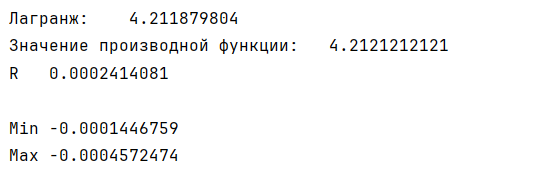
\includegraphics[width=0.5\textwidth]{lab_3_2.png}
    \label{fig:my_label}
\end{figure}

\thispagestyle{empty} 
\newpage
\mbox{}
\thispagestyle{empty} 
\newpage
 
\end{document}

